\documentclass{beamer}
%
% Choose how your presentation looks.
%
% For more themes, color themes and font themes, see:
% http://deic.uab.es/~iblanes/beamer_gallery/index_by_theme.html
%
\mode<presentation>
{
  \usetheme{Madrid}      % or try Darmstadt, Madrid, Warsaw, ...
  \usecolortheme{crane} % or try albatross, beaver, crane, ...
  \usefonttheme{default}  % or try serif, structurebold, ...
  \setbeamertemplate{navigation symbols}{}
  \setbeamertemplate{caption}[numbered]
  
} 

\usepackage[english]{babel}
\usepackage[utf8x]{inputenc}
\usepackage{courier}
\usepackage{dsfont}
\usepackage{verbatim} 
\usepackage{tikz}
\usepackage{caption}
\usepackage{multirow}
\usepackage{venndiagram}
\usepackage{xcolor}
\usepackage{enumitem}
\usepackage{listings}
\usepackage{hyperref}
\hypersetup{
    colorlinks=true,
    linkcolor=blue,
    filecolor=magenta,      
    urlcolor=cyan,
}

\newcommand{\code}[1]{\texttt{#1}}

\usetikzlibrary{shapes,decorations,arrows,calc,arrows.meta,fit,positioning}
\tikzset{
    -Latex,auto,node distance =1 cm and 1 cm,semithick,
    state/.style ={ellipse, draw, minimum width = 0.7 cm},
    point/.style = {circle, draw, inner sep=0.04cm,fill,node contents={}},
    bidirected/.style={Latex-Latex,dashed},
    el/.style = {inner sep=2pt, align=left, sloped}
}

\usepackage{listings}
\lstdefinestyle{rstyle}{
	language=R,
    %stringstyle=\color{green},
    %otherkeywords={0,1,2,3,4,5,6,7,8,9},
    %morekeywords={TRUE,FALSE},
    %deletekeywords={data,frame,length,as,character}
    %keywordstyle=\color{blue},
    %commentstyle=\color{cyan},
}

\setitemize{label=\usebeamerfont*{itemize item}%
  \usebeamercolor[fg]{itemize item}
  \usebeamertemplate{itemize item}}

\newcommand{\Mypm}{\mathbin{\tikz [x=1.4ex,y=1.4ex,line width=.1ex] \draw (0.0,0) -- (1.0,0) (0.5,0.08) -- (0.5,0.92) (0.0,0.5) -- (1.0,0.5);}}%

\title[UIowa Biostatistics]{Prospectus title}
\subtitle{and subtitle!}
\author{Collin Nolte}
\date{April 29, 2022}

\begin{document}

\begin{frame}
  \titlepage
\end{frame}

\begin{frame}{Outline}
\begin{itemize}
\item[1.] bdots
  \begin{itemize}
  \item[a.] Methodology
  \item[b.] Updates
  \item[c.] Non-vwp data
  \end{itemize}
\item[2.] Visual World Paradigm
  \begin{itemize}
  \item[a.] Eyetracking data
  \item[b.] Mathematical description
  \item[c.] Sampling and curves
  \end{itemize}
\item[3.] Simulations
  \begin{itemize}
  \item[a.] Saccades
  \item[b.] Oculomotor delay
  \end{itemize}
\end{itemize}
\end{frame}


%
%\begin{frame}{Overview}
%\begin{center}
%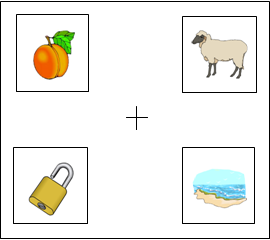
\includegraphics[scale=0.4]{img/visual_world_display.png}
%\end{center}
%\end{frame}

\begin{frame}{bdots}

The idea behind bdots (bootstrapped difference in time series) was originally proposed by Oleson, Cavanaugh, McMurray and Brown (2017) \newline \\

First packaged version for CRAN written by Michael Seedorff, with subsequent updates made by Brad Loeffler \newline \\


\end{frame}

\begin{frame}{bdots}
Current implementation of \code{bdots} involves two steps:
\begin{enumerate}
\item[1.] \textbf{Curve Fitting:} Fitting parametric curve to observed data
\item[2.] \textbf{Bootstrap} Bootstrap curves to estimate group population curve \newline
\end{enumerate}
Additionally, there functions available to assist with refitting poorly fit curves, either with a manual refitting or batch uploading of new starting parameters
\end{frame}

\begin{frame}{Fitting Process}
The current method employed by \code{bdots} is to fit for each observed subject, $y_{it}$, an underlying curve $f_{\theta}$, the fitting step given by 
  \begin{align*}
  F: \{y\} \times f \rightarrow N \left(\hat{\theta}_i, \hat{\Sigma}_{\theta_i} \right)
  \end{align*}

Such that
  \begin{align*}
  \hat{\theta}_i = \text{argmin}_{\theta} \  ||y_{it} - f_{\theta}(t)||^2
  \end{align*}

\end{frame}


\begin{frame}{Bootstrapping Process}
Here, we perform $B$ bootstraps of the subject parameters to construct bootstrapped curves and confidence intervals. Taking parameter estimates from the fitting step, for each subject we draw $B$ samples of $\hat{\theta}_i$, where 
\begin{align*}
\hat{\theta}_{ib} \sim N \left(\hat{\theta_i},  \Sigma_{\hat{\theta}_i} \right)
\end{align*}
resulting in a $B\times p$ matrix, denoted $M_i$. \newline 

Doing this for each subject, we construct a $B\times p$ matrix of the average of bootstraps across iterations, 
\begin{align*}
\overline{M} = \frac1n \sum_{i}^n M_i
\end{align*}
\end{frame}

\begin{frame}{Bootstrapping, cont.}
$\overline{M}$ is again a $B \times p$ matrix, each row  representing the average parameter estimate of $\theta$ at each bootstrap $b$. \newline 

Each $1\times p$ row of $\overline{M}$ returns a $1 \times T$ vector representing estimations of $f_{\theta}$ at each point $t$. Together, we have the $B \times T$ matrix $\overline{M}_f$. This gives an estimated fixation curve, 
\begin{align*}
\hat{f} = \frac1B \sum_{b=1}^B \overline{M}_{\{b, \cdot\}_f}, \qquad \widehat{\text{se}}_{f} = \left[ \frac{1}{B-1} \sum_{b=1}^B \left( \overline{M}_{\{b, \cdot\}_{f}} - \hat{f} \right)^2 \right]^{1/2} 
\end{align*}
\end{frame}



\begin{frame}{Updates}
Fitting process has been simplified to a single function, \texttt{bdotsFit} which can accept arbitrary functions provided by the user, as well as an arbitrary number of experimental groups or conditions \newline

Object returned by \texttt{bdotsFit} are of class \texttt{bdObj}, inheriting from \texttt{data.frame} class \newline

Introduction of a number of useful generics including \texttt{plot}, \texttt{summary}, \texttt{coef}, etc., \newline 

Formula definition introduced in bootstrapping step, removing need to prespecify differences or differences of differences between curves \newline 

Refitting step is interactive, can upload external data, saves progress \newline 

\end{frame}



\begin{frame}[fragile]{Fitting with \texttt{bdots}}
\lstset{basicstyle=\footnotesize\ttfamily, style = rstyle}
\begin{lstlisting}[language=R, showstringspaces=false,deletekeywords={data,col,time,c,}]
## Old bdots
fit0 <- doubleGauss.fit(
  data = dat, # Requires columns "Subject", "Time", and "Group
  col = 4, # Specify outcome with numeric position
  concave = TRUE, # argument tied to curve function
  diffs = TRUE) # Requires column "Curve" with values 1,2
  
## New bdots
fit <- bdotsFit(data = dat,
  subject = "Subject",
  time = "Time",
  y = "Fixations",
  group = c("Group", "LookType"),
  curveType = doubleGauss(concave = TRUE))
\end{lstlisting}
\end{frame}

\begin{frame}[fragile]{Output (old)}
\lstset{basicstyle=\tiny\ttfamily, style = rstyle}
\begin{lstlisting}[language=R, showstringspaces=false,deletekeywords={data,col,time,c,factor, summary, numeric,table,list,coef, all, model, logical, character}]
> summary(fit0)
             Length Class      Mode     
data           7    data.table list     
col            1    -none-     numeric  
rho.0          1    -none-     numeric  
N.time         1    -none-     numeric  
N.sub1         1    -none-     numeric  
N.sub2         1    -none-     numeric  
coef.id1     150    -none-     numeric  
coef.id2     150    -none-     numeric  
sdev.id1     150    -none-     numeric  
sdev.id2     150    -none-     numeric  
sigma.id1     25    -none-     numeric  
sigma.id2     25    -none-     numeric  
coef.id3     150    -none-     numeric  
coef.id4     150    -none-     numeric  
sdev.id3     150    -none-     numeric  
sdev.id4     150    -none-     numeric  
sigma.id3     25    -none-     numeric  
sigma.id4     25    -none-     numeric  
id.nums.g1    25    factor     numeric  
id.nums.g2    25    factor     numeric  
groups         2    -none-     numeric  
time.all     501    -none-     numeric  
N.g1           1    -none-     numeric  
N.g2           1    -none-     numeric  
concave        2    -none-     logical  
model          1    -none-     character
R2.g1.1       25    -none-     numeric  
R2.g2.1       25    -none-     numeric  
R2.g1.2       25    -none-     numeric  
R2.g2.2       25    -none-     numeric  
diffs          1    -none-     logical  
cor            1    -none-     logical  
cor.1         25    -none-     logical  
cor.2         25    -none-     logical  
cor.3         25    -none-     logical  
cor.4         25    -none-     logical  
sdev.id1.cov  25    -none-     list     
sdev.id2.cov  25    -none-     list     
sdev.id3.cov  25    -none-     list     
sdev.id4.cov  25    -none-     list     
\end{lstlisting}
\end{frame}

\begin{frame}[fragile]{Output (new)}
\lstset{basicstyle=\footnotesize\ttfamily, style = rstyle}
\begin{lstlisting}[language=R, showstringspaces=false,deletekeywords={data,col,time,c,}]
> head(fit, n = 15)
    Subject Group LookType        fit      R2   AR1 fitCode
 1:       1    50   Cohort <gnls[18]> 0.96972  TRUE       0
 2:       1    65   Cohort <gnls[18]> 0.98049  TRUE       0
 3:       2    50   Cohort <gnls[18]> 0.98117  TRUE       0
 4:       2    65   Cohort <gnls[18]> 0.96975  TRUE       0
 5:       3    50   Cohort <gnls[18]> 0.97619  TRUE       0
 6:       3    65   Cohort <gnls[18]> 0.95349 FALSE       3
 7:       4    50   Cohort <gnls[18]> 0.97079  TRUE       0
 8:       4    65   Cohort <gnls[18]> 0.64374 FALSE       5
 9:       5    50   Cohort <gnls[18]> 0.97876  TRUE       0
10:       5    65   Cohort <gnls[18]> 0.97656  TRUE       0
11:       6    50   Cohort <gnls[18]> 0.93516  TRUE       1
12:       6    65   Cohort <gnls[18]> 0.92825  TRUE       1
13:       7    50   Cohort <gnls[18]> 0.84164  TRUE       1
14:       7    65   Cohort <gnls[18]> 0.93777  TRUE       1
15:       8    50   Cohort <gnls[18]> 0.98621  TRUE       0
\end{lstlisting}
\end{frame}

\begin{frame}[fragile]{Bootstrap with \texttt{bdots}}
\lstset{basicstyle=\footnotesize\ttfamily, style = rstyle}
\begin{lstlisting}[language=R, showstringspaces=false,deletekeywords={data,col,time,c,list}]
## Old bdots
boot0 <- doubleGauss.boot(
  part1.list = fit0, 
  paired = TRUE) # Must indicate if observations paired
  
## New bdots
boot <- bdotsBoot(
  Fixations ~ Group(50, 65) + LookType(Cohort), 
  bdObj = fit)
  
boot <- bdotsBoot(
  diffs(Fixations, Group(50, 65)) ~ LookType(Cohort, Unrelated), 
  bdObj = fit)
\end{lstlisting}
\end{frame}

\begin{frame}[fragile]{Non-vwp data}
Data for 451LuBR cell line (metastatic melanoma) growth with repeated measures in mice with five treatment groups \newline \\

\lstset{basicstyle=\footnotesize\ttfamily, style = rstyle}
\begin{lstlisting}[language=R, showstringspaces=false,deletekeywords={data,col,time,c,}]
## Using custom curve for fitting data
fit <- bdotsFit(data = dat, 
                subject = "ID", 
                time = "Day", 
                y = "Volume", 
                group = "Treatment", 
                curveType = expCurve())
\end{lstlisting}
\end{frame}

\begin{frame}{Plots}
Representative curves for individual mice, as well as comparisons between two treatments with bootstrapped curves
\begin{columns}
\begin{column}{0.45\textwidth}
\begin{center}
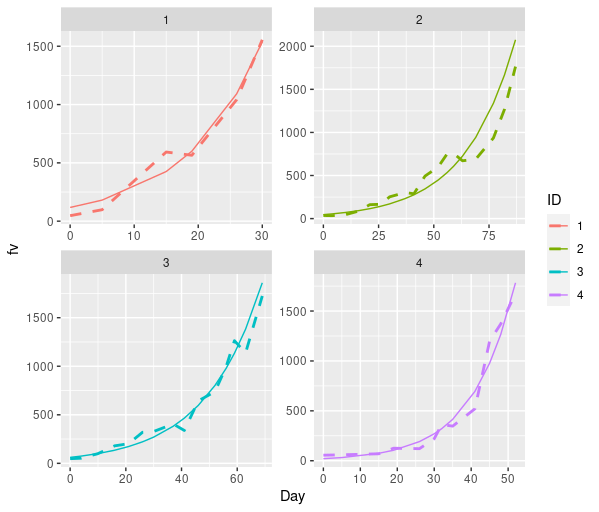
\includegraphics[scale=0.45]{img/tumr_fit.png}
\end{center}
\end{column}
\begin{column}{0.5\textwidth}  %%<--- here
\begin{center}
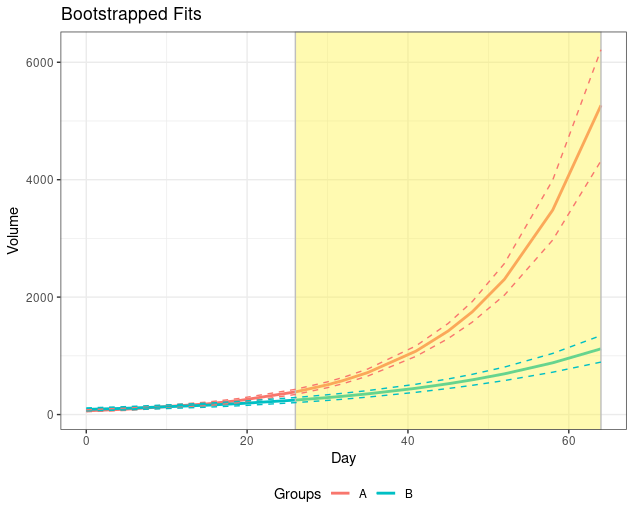
\includegraphics[scale=0.3]{img/tumr_boot.png}
\end{center}
\end{column}
\end{columns}
\end{frame}

\begin{frame}{Other comparisons}
\begin{center}
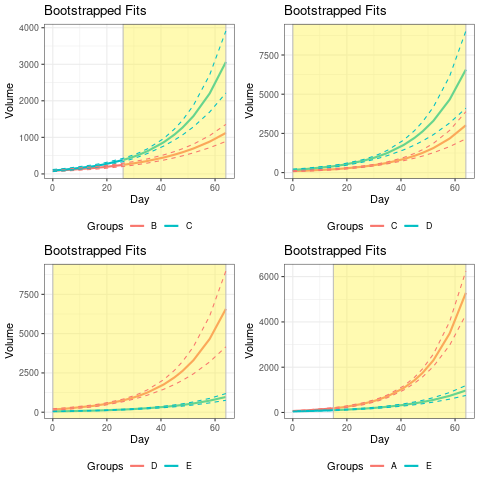
\includegraphics[scale=0.45]{img/four_boot.png}
\end{center}
\end{frame}


\begin{frame}{Future work}
Making package more robust to different types of data \newline 

Handling inconsistencies in time of observations \newline 

Investigate different optimization methods for improving fitted curves \newline 

Convenience functions \newline

\end{frame}

\begin{frame}{Visual World Paradigm}
Broadly speaking, the visual world paradigm (vwp) is a paradigm in which subjects are placed in a ``visual world" in which they are prompted to select an item in response to spoken language \newline \\

Eyetracking software collects location of eye movement in real time as it responds to spoken language \newline \\

``An increasingly popular approach to visual world data is to fit some nonlinear function of time to visualizations of the data...as descriptors of how the trajectories change over time" (Oleson, 2017) \newline \\

%This leads to the idea of using eyetracking data to construct a \textit{fixation curve}, a (typically) parametric function fit to the data collected


\end{frame}

\begin{frame}{Eyetracking data}

Two types of events make up eyetracking data: \textit{saccades} and \textit{fixations} \newline \\

A \textit{saccade} represents the physical movement of an eye, lasting between 20-200ms. There is also about a 200ms oculomotor delay between planning an eye movement and it occuring \newline \\

A \textit{fixation} is characterized by a lack of movement, in which the eye is fixated on a particular location. The length of a fixation is more  variable \newline \\

Together, a saccade, followed by a subsequent fixation, is known as a \textit{look}
\end{frame}

\begin{frame}{Saccade, Fixations, and Looks (oh my!)}
\vspace{10mm}
\begin{center}
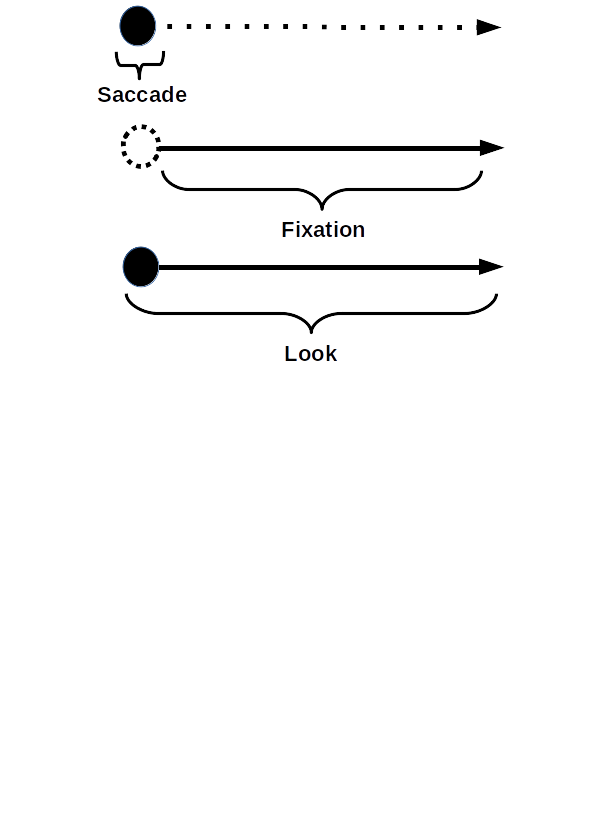
\includegraphics[scale=0.45]{img/saccade_def2.png}
\end{center}
\end{frame}


%\begin{frame}{Fixation curve}
%We define a \textit{fixation curve}, $f_{\theta}(t)$ or $f(t  | \theta)$ to represent a (usually parametric) function indicating the probability of fixating on a target at some time, $t$. \newline \\
%To disambiguate the term ``target" when used in the VWP, we will let ``Target" denote the object corresponding to a spoken word, while ``target" will denote an object of interest \newline \\
%
%For example, with the four-parameter logistic, our target is typically the Target, while for the six-parameter double-gauss, our target is the Cohort
%\end{frame}



\begin{frame}{Aggregation of Data}
\begin{columns}
\begin{column}{0.5\textwidth}
Subjects are measured across a series of trials in which they are asked to identify the Target \newline 

Fixations are captured in real time and aggregated across trials, with each time point representing the proportions of trials in which a subject was fixed on any item \newline 

The resulting proportion of fixations then serves as the empirical observation of the \textit{fixation curve}, a (usually parametric) function indicating the probability of fixating on a target at some time, $t$.
\end{column}
\begin{column}{0.5\textwidth}  %%<--- here
\begin{center}
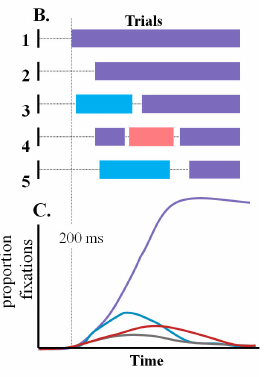
\includegraphics[scale=0.5]{img/bob_aggregate.png}
\\
{\tiny source: Princess Bride paper}
\end{center}
\end{column}
\end{columns}
\end{frame}

\begin{frame}{Mathematical Expression of Aggregate Data}
For subjects $i = 1, \dots, n$, trials $j = 1, \dots, J$, and time points $t = 1, \dots, T$, the current method of estimating this curve is 

\begin{align*}
y_{it} = \frac{1}{J} \sum_{j=1}^J z_{ijt}
\end{align*}
where $z_{ijt} = \{0,1\}$, conditional on the measured fixation at timepoint $t$ in trial $j$. \newline \\

Here, the vector $y_i$ serves as a direct observation of $f_{\theta}(t)$ for subject $i$ 
\end{frame}

\begin{frame}{What's in a name?}
Briefly, we need to address the fact that there are a few distinct but similar ``curves" in question here \newline \\

First, there is what we might call an ``activation" curve, representing some latent mental process corresponding to activation of a word \newline \\

There are also empirical fixation ``curves", either a set of discrete fixations for a single trial, or the proportions of fixations, aggregated at each time point \newline \\

Finally, we have the idealized ``looking" curve, the (possibly parametric) curve indicating the probability of fixating on a target at a particular time \newline \\

Still unsettled
\end{frame}

\begin{frame}{VWP and looks}
Of critical importance here are the underlying assumptions relating cognitive activation of an object and the resulting fixations, referred to as a grounding hypothesis (Magnuson 2019) \newline \\

We can begin by assuming that there is some underlying function dictating fixations, though how this is mediated with observed data is still up for debate \newline \\

Bob explored a number of these assumptions in his Princess Bride paper (\textit{Fixation Curves in the Visual World Paradigm}, 2022?), and here we will focus on two: high frequency sampling and fixation-based sampling, augmented for target

\end{frame}


\begin{frame}{Sampling Paradigms}

\textbf{HFS:} High frequency sampling assumption, "if researcher is sampling at 4ms intervals, the fixation curve is assumped to derive from a probabilistic sample every 4ms" \newline 

\textbf{FBS+T:} Fixation-based sampling + target, series of discrete fixations with reasonable refractory period, treats fixations as primarily a readout ouf the unfolding decision, ignores the role of the fixation as an information gather behavior, allows fixations to target to be slightly longer (once fixated, subject more likely to stay)
\end{frame}

\begin{frame}{Why do we care?}

The differences in sampling assumptions raises questions as to biases introduced in our estimate of the fixation curve. \newline

\begin{itemize}
  \item[-] Can each observed time point be considered an independent draw from a fixation curve?
  \item[-] How do the lengths of each fixation impact potential bias?
  \item[-] Does the duration of these fixations change over time and in response to previously identified items?
\end{itemize}

\vspace{4mm}

With recovery of the underlying fixation curve being our goal, we should be able to recover the underlying curve from observed data according to a particular hypothesis \newline 

\end{frame}

\begin{frame}{High Frequency Sampling}

On the positive side, simulations run with the HFS assumption were able to correctly recover the underlying fixation curve \newline \\

As Bob has noted, however, the HFS assumption is ``patently untrue" \newline \\

While the bdots package was originally created as a means of modeling the data to account for autocorrelation, it is unable to take into consideration the dynamics of fixations \newline \\


We will then limit our attention to FBS+T in consideration of potential biases introduced by the mechanics of eye movement

\end{frame}

%\begin{frame}{High Frequency Sampling}
%On the positive side, simulations run with the HFS assumption were able to correctly recover the underlying fixation curve \newline \\
%
%As Bob has noted, however, the HFS assumption is ``patently untrue" \newline \\
%
%While the bdots package was originally created as a means of modeling the data to account for autocorrelation, it is unable to take into consideration the dynamics of fixations \newline \\
%
%We will then limit our attention to FBS+T in consideration of potential biases introduced by the mechanics of eye movement
%
%
%\begin{tikzpicture}[remember picture,overlay]
%\node at (current page.center){
\includegraphics[scale=0.5]{img/gump.jpeg}};
%\end{tikzpicture}
%\end{frame}

\begin{frame}{FBS+T}
Fixation based sampling introduces a more realistic situation in which looks to a particular target are initiated at some point, but then remain fixated for a random period of time \newline \\

Empirically, fixations on the target tend to last longer than others, adding an additional mechanic to the generation of data \newline \\

Finally, there is the adjustment for oculomotor delay; when a saccade occurs at 1200ms, it is likely that it was planned around 1000ms \newline \\


\end{frame}

%
%\begin{frame}[fragile]
%\frametitle{current simulation (fbs+t)}
%Begin by creating a subject \newline \\
%
%  \begin{enumerate}
%  \item[1.] Draw $\theta \sim N(\theta^*, \Sigma_{\theta^*})$ s.t $max(f_{\theta}) \in (0.6, 1)$
%  \item[2.] Draw parameters from distribution $\Gamma$ for duration of fixation to non-target
%  \item[3.] Draw parameters for distribution $\Gamma_T$ for duration of fixation to Target
%  \item[4.] Return $(\theta, \Gamma, \Gamma_T)$
%  \end{enumerate}
%
%\end{frame}
%
%\begin{frame}{Current sim (fbs+t)}
%Single trial. With vector of times, \code{time}, run the following simulation:\newline \\
%
%\code{pars <- makeSubject()} \\
%\code{currTime <- min(time) - runif(1)}$E(\Gamma)$ \\
%\code{lastTime <- currTime - }$\Gamma$\code{ - runif(1)}$E(\Gamma)$\newline \\
%\code{while(currTime < max(time)) \{} \\
%\hspace{4mm} \code{p <- f(lasttime|}$\theta$\code{)} \\
%\hspace{4mm} \code{target <- runif(1) < p} \\
%\hspace{4mm} \code{duration <- ifelse(target, }$\Gamma$\code{, }$\Gamma_T$\code{)} \\
%\hspace{4mm} \code{lasttime <- currTime} \\
%\hspace{4mm} \code{currTime <- currTime + duration} \\
%\code{\}}
%\end{frame}

\begin{frame}{Simulations}
Simulations were run with a single subject with $N = 300$ trials \newline \\

Following FBS+T to generate eyetracking data \newline \\

Plots include the data generating curve, observed data from the simulation, estimated curve with bdots, along with second bdots curve with 200ms oculomotor shift \textit{prior} to fitting

\end{frame}

\begin{frame}{FBS+T}
\begin{center}
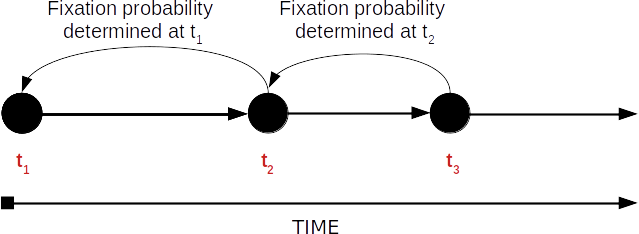
\includegraphics[scale=0.45]{img/occulomotor_delay_1.png}
\end{center}
\end{frame}

\begin{frame}{FBS+T plot}
\begin{center}
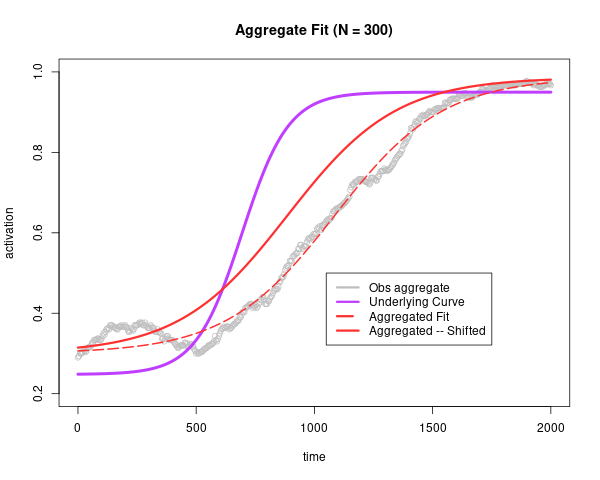
\includegraphics[scale=0.45]{img/aggregate_fit_only.png}
\end{center}
\end{frame}

\begin{frame}{Fixation vs Saccade}
Here, we reflect again on the construction of our empirical fixation curve, 

\begin{align*}
y_{it} = \frac1J \sum_{j=1}^J z_{ijt}.
\end{align*}

Critically, we realize that the only sample from the fixation curve that we observe \textit{is at the saccade}. \newline \\

In other words, if the subject fixates on the target at $t$ for 500ms, we have introduced ``observed" data through $(t+1, t + 500)$ from a sample of the fixation curve taken at time $t$
\end{frame}


\begin{frame}{Aggregate vs Saccade}
\begin{center}
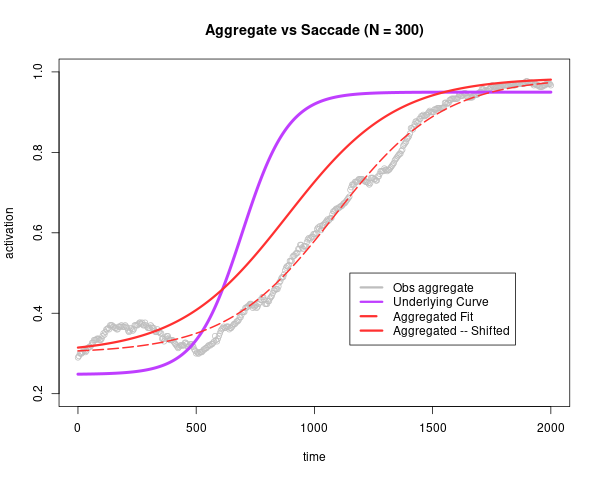
\includegraphics[scale=0.45]{img/aggregate_sac_1.png}
\end{center}
\end{frame}

\begin{frame}{Aggregate vs Saccade}
\begin{center}
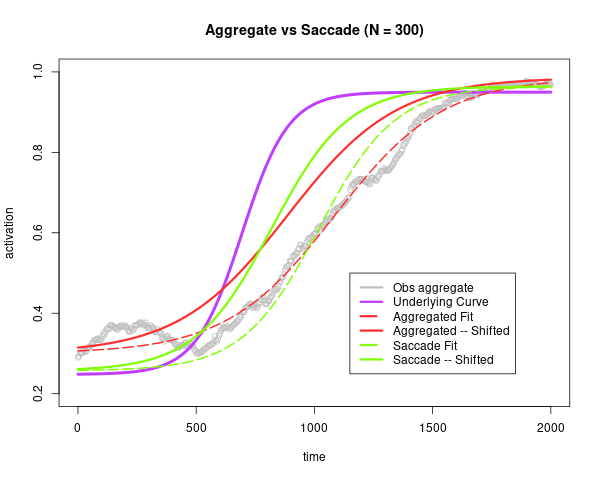
\includegraphics[scale=0.4]{img/aggregate_sac_2.png}
\end{center}
% latex table generated in R 4.1.3 by xtable 1.8-4 package
% Wed Apr 27 15:30:52 2022
{\scriptsize
\begin{table}[H]
\captionsetup{font=scriptsize}
\centering
\begin{tabular}{rccccc}
  \hline
 & Aggregate & Saccade  & Aggregate -- Shifted & Saccade -- Shifted & Underlying \\ 
  \hline
MISE & 21.96 & 19.34
& 5.04 & 1.77 & 0.00 \\ 
   \hline
\end{tabular}
\end{table}
}
\end{frame}

\begin{frame}{Asymptotic}
\begin{center}
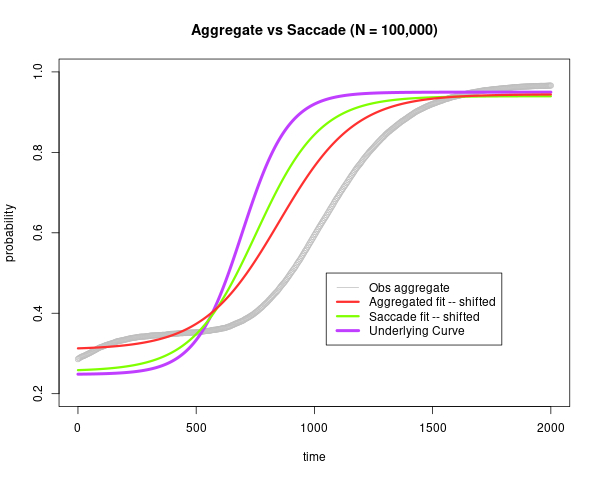
\includegraphics[scale=0.45]{img/asy_fit.png}
\end{center}
\end{frame}

\begin{frame}{Adjusting Occulomotor Delay}
\begin{center}
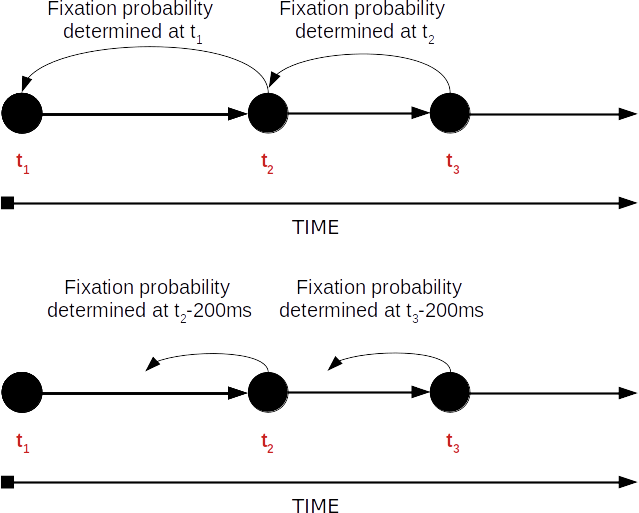
\includegraphics[scale=0.4]{img/occulomotor_delay_2.png}
\end{center}
\end{frame}

\begin{frame}{200ms delay}
\begin{center}
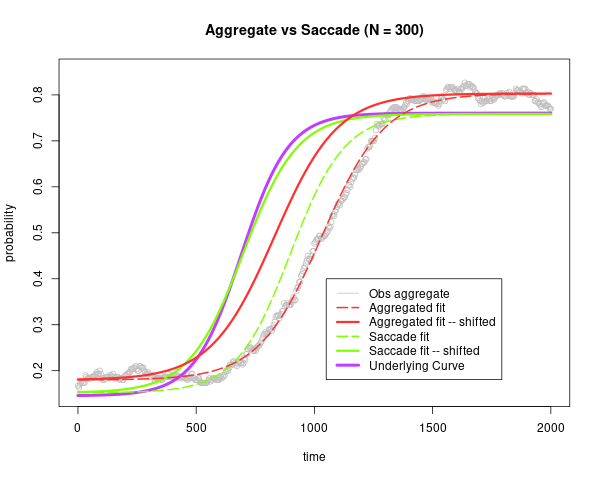
\includegraphics[scale=0.45]{img/new_delay1.png}
\end{center}
\end{frame}

\begin{frame}{200ms delay}
\begin{center}
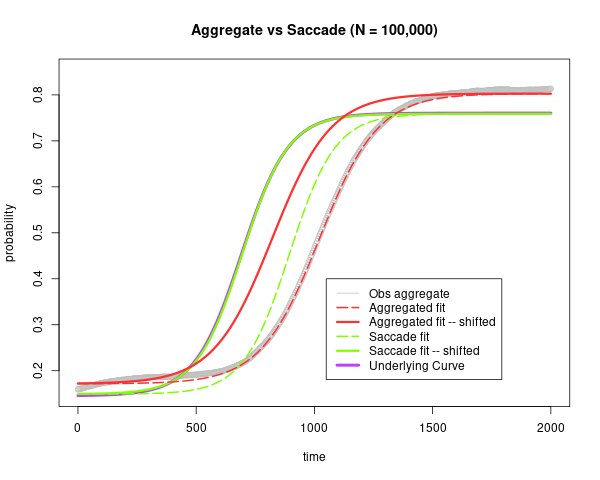
\includegraphics[scale=0.45]{img/new_delay2.png}
\end{center}
\end{frame}

\begin{frame}{Future Directions?}
Revist fitting/refitting process to make more robust to bad fits \newline \\

Investigate bootstrap confidence intervals for correct coverage \newline \\

Consideration of nonparametric fits for data \newline \\

Window/variability theory \newline \\

``Information gathering behavior"
\end{frame}

%\begin{frame}{identity theroem and time windows}
%The identity theorem for analytic functions states: given functions $f$ and $g$ analytic on (open and connected) domain $D$, if $f = g$ on some $S \subseteq D$, where $S$ has an accumulation point, then $f = g$ on $D$ (wikipedia) \newline \\
%
%In other words, letting $D$ be time, if we were able to identify values $\hat{\theta}$ such that $f_{\hat{\theta}} = f_{\theta}$  some interval $S$, then we should find that $f_{\hat{\theta}} = f_{\theta}$ on $D$ \newline \\
%
%In other words again, if we could identify some interval where our approximation of $f$ was best, we could extrapolate this for the rest of the domain
%\end{frame}


%\begin{frame}{other issues}
%Density of saccades over time \newline \\
%identity theorem \newline \\
%still does 0-2000ms (how to deal with identifying target/RT) \newline \\
%``Ignores the role of the fixation as an information gathering behavior" \newline \\
%
%Can show sims demonstrating time/density/etc with saccades and  wolololo
%\end{frame}



%\begin{frame}{Limitations}
%Not really recovering cognitive curve \newline 
%
%Assumes that all trials are drawn from the same functional curve (that is, independent of trial conditions) \newline 
%
%\end{frame}

\begin{frame}{References}
Magnuson, James S. \textbf{Fixations in the visual world paradigm: where, when, why?} 2019-09 \textit{Journal of Cultural Cognitive Science}, Vol. 3, No. 2 Springer  Science and Business Media LLC p. 113-139 \newline \\

McMurray, Bob \textbf{Fixation Curves in the Visual World Paradigm} 2020 \newline \\

Oleson, Jacob J / Cavanaugh, Joseph E, McMurray, Bob / Brown, Grant \textbf{Detecting time-specific differences between temporal nonlinear curves: Analyzing data from the visual world paradigm} 2017 \textit{Statistical Methods in Medical Research}, Vol. 26, No. 6 p 2708-2725 \newline \\
\end{frame}

\end{document}